\documentclass[paper=a4, fontsize=11pt]{scrartcl} % A4 paper and 11pt font size

\usepackage[T1]{fontenc} % Use 8-bit encoding that has 256 glyphs
\usepackage{fourier} % Use the Adobe Utopia font for the document - comment this line to return to the LaTeX default
\usepackage[english]{babel} % English language/hyphenation
\usepackage{amsmath,amsfonts,amsthm} % Math packages
\usepackage{graphicx}

\usepackage{lipsum} % Used for inserting dummy 'Lorem ipsum' text into the template

\usepackage{sectsty} % Allows customizing section commands
\allsectionsfont{\centering \normalfont\scshape} % Make all sections centered, the default font and small caps

\usepackage{fancyhdr} % Custom headers and footers
\pagestyle{fancyplain} % Makes all pages in the document conform to the custom headers and footers
\fancyhead{} % No page header - if you want one, create it in the same way as the footers below
\fancyfoot[L]{} % Empty left footer
\fancyfoot[C]{} % Empty center footer
\fancyfoot[R]{\thepage} % Page numbering for right footer
\renewcommand{\headrulewidth}{0pt} % Remove header underlines
\renewcommand{\footrulewidth}{0pt} % Remove footer underlines
\setlength{\headheight}{13.6pt} % Customize the height of the header



\numberwithin{equation}{section} % Number equations within sections (i.e. 1.1, 1.2, 2.1, 2.2 instead of 1, 2, 3, 4)
\numberwithin{figure}{section} % Number figures within sections (i.e. 1.1, 1.2, 2.1, 2.2 instead of 1, 2, 3, 4)
\numberwithin{table}{section} % Number tables within sections (i.e. 1.1, 1.2, 2.1, 2.2 instead of 1, 2, 3, 4)

\setlength\parindent{0pt} % Removes all indentation from paragraphs - comment this line for an assignment with lots of text

%----------------------------------------------------------------------------------------
%       TITLE SECTION
%----------------------------------------------------------------------------------------

\newcommand{\horrule}[1]{\rule{\linewidth}{#1}} % Create horizontal rule command with 1 argument of height

\title{
\normalfont \normalsize
\textsc{Jiangsu University, school of Computer Science and Communication Engineering} \\ [25pt] % Your university, school and/or department name(s)
\horrule{0.5pt} \\[0.4cm] % Thin top horizontal rule
\huge Exercises \\ % The assignment title
\horrule{2pt} \\[0.5cm] % Thick bottom horizontal rule
}

\author{AiLan Wan} % Your name

\date{\normalsize\today} % Today's date or a custom date

\begin{document}

\maketitle % Print the title
\section{Digital signature}
\label{sec:ds}
\subsection{Digital signature Problem \uppercase\expandafter{\romannumeral1}}

\textbf{1.}Please introduce the basic principle and process of digital signature briefly.
\\
\\
\textbf{Answer:}
\\
\\
Digital signature is different from encryption.Its main purpose is to ensure the integrity and authenticity of the data,it generally consists of two parts:Signature algorithm and verification algorithm,usually by the public key cryptography and hash function (Hash algorithm) combined to achieve.Assuming that sender $A$ wants to send a message $M$ to recipient $B$, and the message is digitally signed, its concrete principle and process are as follows:
\begin{enumerate}
\item Sender $A$ uses the hash function to generate the message to send message $M$ Summary: Hash($M$);
\item The sender $A$ encrypts the message digest of the message $M$ with its own private key $P$ and realizes the signature: $E_P$(Hash($M$)) and concatenates the message with the message $M$ to form the message to be finally sent: $M$||$E_P$(Hash($M$)), and then sends the message;
\item After receiving the message, receiver $B$ decrypts the signature using the public key $P$ of sender $A$ to restore the digest of the original message: Hash($M$)= $D_P$(Hash($M$)));
\item Recipient $B$ uses the hash function to recalculate the message digest: Hash($M$) of message $M$ and compares it with the message digest received from sender $A$. If it is equal, The message is indeed sent by sender $A$, and the contents of the message have not been modified. Digital signature technology plays an important role in network security communications and the success of various electronic trading systems.
\end{enumerate}

\textbf{2.}What are the properties a digital signature should have?
\\
\\
\textbf{Answer:}
\begin{enumerate}
\item It must be able to verify the author and the date and time of the signature.
\item It must be able to authenticate the contents at the time of the signature.
\item The signature must be verifiable by third parties, to resolve disputes.
\end{enumerate}

\textbf{3.}What requirements should a digital signature scheme satisfy?
\\
\\
\textbf{Answer:}
\begin{enumerate}
\item The signature must be a bit pattern that depends on the message being signed.
\item The signature must use some information unique to the sender, to prevent both forgery and denial.
\item It must be relatively easy to produce the digital signature.
\item It must be relatively easy to recognize and verify the digital signature.
\item It must be practical to retain a copy of the digital signature in storage.
\end{enumerate}

\textbf{4.}In what order should the signature function and the confidentiality function be applied to a message, and why?
\\
\\
\textbf{Answer:}
\begin{enumerate}
\item It is important to perform the signature function first and then an outer confidentiality function.
\item In case of dispute, some third party must view the message and its signature.
\item If the signature is calculated on an encrypted message, then the third party also needs access to the decryption key to read the original message.
\item However, if the signature is the inner operation, then the recipient can store the plaintext message and its signature for later use in dispute resolution.
\end{enumerate}

\textbf{5.}An early proposal for a digital signature scheme using symmetric encryption is based on the following. To sign an message, the sender randomly generates in advance $56$ bit cryptographic keys:$k_1$,$K_1$,$k_2$,$K_2$,\ldots, $k_n$,$K_n$, which are kept private. The sender prepares in advance two sets of corresponding non-secret 64-bit validation parameters, which are made public:$u_1$,$U_1$,$u_2$,$U_2$,\ldots, $u_n$,$U_n$, and $v_1$,$V_1$,$v_2$,$V_2$, \ldots, $v_n$,$V_n$, where $V_i$ = $E$($k_i$,$u_i$),$V_i$ = $E$($K_i$,$U_i$). The message is signed as follows. For the message, either or is attached to the message, depending on whether the message bit is $0$ or $1$. For example, if the first three bits of the message are $011$, then the first three keys of the signature are $k_1$,$K_2$,$K_3$.
\\
\\
\textbf{Question:}
\begin{enumerate}
\item How does the receiver validate the message?
\item Is the technique secure?
\item How many times can the same set of secret keys be safely used for different messages?
\item What, if any, practical problems does this scheme present?
\end{enumerate}

\textbf{Answer:}
\begin{enumerate}
\item The receiver validates the digital signature by ensuring that the first $56$ bit key in the signature will encipher validation parameter $u_1$ into $E$($k_1$,$u_1$) if the first bit of $M$ is $0$, or that it will encipher $U_1$ into $E$($K_1$,$U_1$) if the first bit of $M$ is $1$; the second $56$ bit key in the signature will encipher validation parameter $u_2$ into $E$($k_2$,$u_2$) if the second bit of $M$ is $0$, or it will encipher $U_2$ into $E$($K_2$,$U_2$) if the second bit of $M$ is $1$.
\item Only the sender, who knows the private values of $k_i$ and $K_i$ and who originally creates $v_i$ and $V_i$ from $u_i$ and $U_i$ can disclose a key to the receiver. An opponent would have to discover the value of the secret keys from the plaintext-ciphertext pairs of the public key, which was computationally infeasible at the time that $56$ bit keys were considered secure.
\item This is a one-time system, because half of the keys are revealed the first time.
\item A separate key must be included in the signature for each bit of the message resulting in a huge digital signature.
\end{enumerate}

\textbf{6.}In the digital signature algorithm DSA, if the random number $k$ is leaked, what will happen?
\\
\\
\textbf{Answer:}
\begin{enumerate}
\item If the value of $k$ used in the DSA signature is leaked, since $s$ = $k^{-1}$(H($m$)+$xr)$ mod $q$, the remaining parameters except $x$ are known.
\item From the binary indefinite congruence equation to the univalent congruence equation of $x$, the private key $x$ can be obtained, so the attacker can forge the signature of any message.
\end{enumerate}

\textbf{7.}What is the difference between direct digital signatures and arbitrable digital signatures?
\\
\\
\textbf{Answer:}
\begin{enumerate}
\item A direct digital signature is a digital signature that involves only the two sides of the communication. In order to provide the authentication function, a direct digital signature generally uses a public key
    cryptosystem.
\item The arbitrable digital signature introduces the mediator's participation on the basis of both parties.
\item It is common practice for all signature messages from sender $X$ to receiver $Y$ to be sent first to arbiter $A$, $A$ to perform a series of tests on the message and its signature to examine its origin and content, and then to date the message and sent to $Y$ along with the signature that has been validated by the arbitrator.
\item Arbitrators play a referee role in this type of signature model. All participants must be absolutely certain that this arbitration mechanism is working properly.
\end{enumerate}

\textbf{8.}Consider the problem of creating domain parameters for DSA.Suppose we have already found primes $p$ and $q$ such that $q$|$(p-1)$. Now we need to find $g \in Z_p$ with $g$ of order $q$ and $p$.Consider the following two algorithms:
\begin{figure}[htbp]
  \centering
  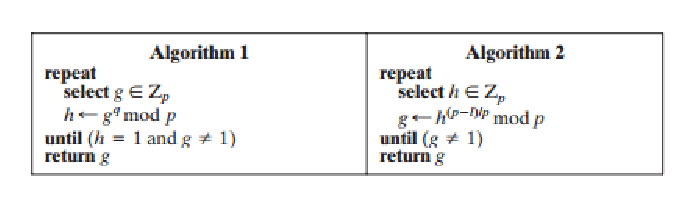
\includegraphics[width=7cm]{1.eps}
  \label{5-1}
\end{figure}
\\
\textbf{Question:}
\begin{enumerate}
\item Prove that the value returned by Algorithm $1$ has order $q$.
\item Prove that the value returned by Algorithm $2$ has order $q$.
\item Suppose $p = 40193$ and $q = 157$. How many loop iterations do you expect Algorithms $1$ to make before it finds a generator?
\item If $p$ is $1024$ bits and $q$ is $160$ bits,would you recommend using Algorithm $1$ to find $g$?
\end{enumerate}

\textbf{Answer:}
\begin{enumerate}
\item If Algorithm $1$ returns the value $g$, then we see that $g^q$ = $1 (mod p)$. Thus, $ord(g)$ divides $q$. Because $q$ is prime, this implies that $ord(g) \in \{1,q\}$. However, because $g \neq  1$, we have that $ord(g) \neq 1$, and so it must be that $ord(g) = q$.
\item If Algorithm $2$ returns the value $g$, then we see that $g^q = 1 mod p$.. Thus, $ord(g)$ divides $q$. Because $q$ is prime, this implies that $ord(g) \in \{1,q\}$. However, because $g \neq 1$, we have that $ord(g) \neq 1$, and so it must be that $ord(g) = q$.
\item Algorithm $1$ works by choosing elements of $Z_p$ until it finds one of order $q$. Since $q$ divides $p-1$, $Z_p$ contains exactly $f(q) = q - 1$ elements of order $q$. Thus, the probability that $g \in Z_p$ has order $q$ is $(q - 1)/(p - 1)$. When $p = 40193$ and $q = 157$ this probability is $156/40192$ . So, we expect Algorithm $1$ to make $40192/156  \approx  258$ loop iterations.
\item No. If $p$ is $1024$ bits and $q$ is $160$ bits, then we expect Algorithm $1$ to require $(q-1)/(p-1)$  = 2$^{854}$  loop iterations.
\end{enumerate}

\textbf{9.}Please give a brief introduction to $RSA$ algorithm signature and verification process.
\\
\\
\textbf{Answer:}\\
\noindent 1.Signing process:\\
\hspace*{0.5cm}(1)\ $A$ computes the message digest of message $m$, denoted by $h$($m$).  \\
\\
\hspace*{0.5cm}(2)\ $A$ uses the private key ($n$,$d$) to encrypt $h(m)$, and generates the signature $s$, $s$ satisfying: $s = (h(m))^ d$ mod $n$; Since $A$ encrypts the message digest with its own private key, Only use the public key to decrypt the message digest, so $A$ can not deny that they sent the message to $B$.  \\
\\
\hspace*{0.5cm}(3)\ $A$ sends the message and signature ($m$,$s$) to $B$.   \\
\\
\noindent 2.Validation process:\\
\\
\hspace*{0.5cm}(1)\ $B$ calculate the message digest of message $m$, denoted by $h(m)$.  \\
\\
\hspace*{0.5cm}(2)\ $B$ decrypts $s$ using public key of $A(n,e)$ to get $H(m)$ = $s ^ e$ mod $n$.  \\
\\
\hspace*{0.5cm}(3)\ $B$ compares $H(m)$ with $h(m)$, the same is proved.   \\

\textbf{10.}For the RSA digital signature scheme, suppose $p = 839$, $q = 983$, $N = p\times q = 824737$. The private key $d = 132111$ is known to calculate the signature of the public key $e$ and the message $m = 23547$.
\\
\\
\textbf{Answer:}
\begin{enumerate}
\item By RSA signature system can be $e$ = $d^{-1}$ mod $ \varphi(N)$ = 132111$^{-1}$ mod $882916=26959$.
\item The signature of the message $s$ = $m^d$ mod $N$ = 23547$^{132111}$ mod $824737=266749$.
\end{enumerate}

\textbf{11.}For the RSA digital signature scheme, assume that modulo $N = 824737$ and public key $e = 26959$.
\\
\\
\textbf{Question:}
\begin{enumerate}
\item Knowing that the signature of the message $m$ is $s = 8798$, find the message $m$.
\item Is the data pair $(m, s) = (167058, 366314)$ a valid message-signature pair?
\item $(M,S) = (629489, 445587)$ and $(m', s') = (203821,229149)$, we need to find the signature of $m \times m'$ for two valid message-signature pairs.
\end{enumerate}

\textbf{Answer:}
\begin{enumerate}
\item By the formula available: $m$=$s^e$ mod $N$ = $8798$$^{26959}$ mod $824737 = 123456$.
\item Since $m'$= $s^e$ mod $N$ = 366314$^{26959}$ mod $824737 = 167058 = m$, it is a valid message-signature pair.
\item The signature of $m \times m'$ is $y = (m \times m') d$ mod $N = s \times s'$ mod $N = 4455587 \times 229149$ mod $824737 = 75915$.
\end{enumerate}

\textbf{12.}For the RSA digital signature scheme, assume that modulo $N = 824737$ and public key $e = 26959$.
\\
\\
\textbf{Question:}
\begin{enumerate}
\item Knowing that the signature of the message $m$ is $s = 8798$, find the message $m$.
\item Is the data pair $(m, s) = (167058, 366314)$ a valid message-signature pair?
\item $(M, s) = (629489, 445587)$ and $(m', s') = (203821,229149)$, we need to find the signature of $m \times m'$ for two valid message-signature pairs.
\end{enumerate}

\textbf{Answer:}
\begin{enumerate}
\item By the formula available: $m$= $s^e$ mod $N$ = $8798^{26959}$ mod $824737 = 123456$.
\item Since $m'= s^e$ mod $N$ = $366314^{26959}$ mod $824737 = 167058 = m$, it is a valid message-signature pair.
\item The signature of $m \times m'$ is $y$ = $(m \times m')$$^ d$ $mod N$ = $s \times s' mod N$ = $4455587 \times 229149$ mod $824737 = 75915$.
\end{enumerate}

\textbf{13.}Suppose that the plaintext information that needs to be encrypted is $m = 14$, choose: $e = 3$, $p = 5$, $q = 11$, explain the encryption and decryption process and result using RSA algorithm.
\\
\\
\textbf{Answer:}
\begin{enumerate}
\item $n = p \times q = 5 \times 11 = 55$, and let $m = (q-1) \times (p-1)$.
\item Find $d$, $ed = 1$ mod $m$. So $d = 27$.
\item Encryption: $Y$ = $m ^ e$ mod $n$ = $14 ^ 3 mod 55 = 49$.
\item Decryption: $X$ = $Y ^ e$ mod $n$ = $49 ^ 27 mod 55 = 14 = m$ decrypted to get the plaintext $m$, proved that the calculation is correct.
\end{enumerate}

\textbf{14.}In the ElGamal digital signature scheme, suppose $p = 11$, $g = 2$ is the primitive of $Z_{11}$, and select $x = 8$, $y = gx$ mod $p = 28$ mod $11$. $P$, $g$, $y$ public, $x$ confidential. Assuming that Alice signs the message $m = 5$ and its secret selection $k = 9$, calculate Alice's signature on $m$ and write out the receiver Bob's verification of the signature.
\\
\\
\textbf{Answer:}
\begin{enumerate}
\item Calculate the public key: $r$ = $g ^ k$ mod $p$ = $29$ mod $11 = 6$, $s$ = $(M-x \times r) k-1$ mod $p-1 =3$.
\item The signer $A$ has an ELGAMAL signature of $M = (6,3)$.
\item The receiver $B$ can verify the signature $(6,3)$ of the message $M = 5$. Because $3^6 \times 6^3 =2^5$ mod $11$.
\end{enumerate}

\textbf{15.}In the ElGamal digital signature scheme, it is assumed that $p = 19$ and $g = 13$. If the private key selected by signer $A$ is $x = 10$, calculate the public key. Let the signer $A$ sign the message $M = 15$, and select the random number $k = 11$, and ask the signer $A$ to sign $M = 15$. And verify the validity of the digital signature.
\\
\\
\textbf{Answer:}
\begin{enumerate}
\item Calculate the public key: $y = gx$ mod $p = 13^10 mod 19 = 6$.
\item Calculate the signature: $r=g^k$ mod $p$ = $13^11$ mod $19$ = $2$, $s$ = $(m-x \times r)$ $k^{-1}$ mod $(p-1)$,so the signature is $(r,s)=(2, 11)$.
\item Since $y ^ r \times $ $r^s$ mod $p$ = 8 = $g^m$ mod $p$ = $13^{15}$ mod $19 = 8$, the signature is valid.
\end{enumerate}

\textbf{16.}Suppose in the ElGamal digital signature system, $p = 31847$, $g = 5$, the public key $y = 25703$. Known $(23972,31396)$ is the signature of the message $M=8990$, $(23972,20481)$ is the signature of the message $M = 31415$,find the random number $k$ and the private key $x$.
\\
\\
\textbf{Answer:}
\begin{enumerate}
\item Since gcd $(10915, 31846) = 1$, we can solve the problem by solving the problem of the same time  as gcd $(10915, 31846)$ =$ k (v-s) = (w-m)$ mod $(p-1)$,$k (31396-20481) = (8990-31415)$ mod $31846$,so $10915k = 9421$ mod $31846$.
\item The residual equation yields: $k = 1165$.
\item We can achieve $23972 \times x = 23704$ mod $31846$,since gcd $(23972, 31846) = 2$.
\item The congruence equation has two solutions, respectively is: $7459$ and $23382$, and then the value of $x$ into the public key $y$ = $g^x$ mod $p$ = $5^x$ mod $31847 = 25703$ in the check that: $x = 7459$.
\end{enumerate}

\textbf{17.}In EIGamal signature scheme, $p = 17$, $g = 2$.
\\
\\
\textbf{Question:}
\begin{enumerate}
\item If select $x = 8$, calculate $y$.
\item If $k = 9$ is selected, please try to sign the message $m = 7$.
\end{enumerate}

\textbf{Answer:}
\begin{enumerate}
\item By $y$ = $g^x$ mod $p$,we can achieve that $y$ = $2^8$ mod $17 =1$.
\item $y = g^k$ mod$ p=29$ mod $17 = 2$,$s = (7-8 \times 2) \times 9^{-1}$ mod $16=15$, so $(2,15)$ is the signature of the message $m = 7$.
\end{enumerate}

\textbf{18.}Please introduce the relationship and difference of three signature schemes, ELGAMAL, SCHNORR and DSA briefly.
\\
\\
\textbf{Answer:}
\begin{enumerate}
\item ElGamal signature is a multiple digital signature, multi-signature is a number of users on the same message for digital signature and authentication.
\item SCHNORR signature is a group signature, in a group signature scheme, a group of any member can be anonymous way on behalf of the entire group to sign the message. As with other digital signatures, group signatures are publicly verifiable, and can be verified using only a single group public key.
\item DSA is a blind signature, blind signature allows the message to blind the first message, and then let the signature of the blinded message signature, the message owner to remove the blind factor signature, get the signer on the original message signature.
\end{enumerate}

\textbf{19.}For the Chaum-van Antwerpen undeniable digital signature protocol, suppose $p = 1019$, $q = 509$, $a = 475$, and private key $x = 200$.
\\
\\
\textbf{Question:}
\begin{enumerate}
\item Find the public key $y$.
\item Find the signature of the message $m = 555$.
\item Select the pair of random numbers $(e1, e2) = (20, 411)$ to verify the validity of the signature.
\end{enumerate}

\textbf{Answer:}
\begin{enumerate}
\item $v=a^s$ mod $p=475200$ mod $1019=807$.
\item Signature $s = m^s$ mod $p = 555^{200}$ mod $1019$.
\item We can achieve $d = c^{x-1}$ mod = $q$ mod $p = 21928$ mod $1019 = 528$, and sends $d$ to the verifier. After verifying $d$ received $d_m  = 528$, verify that $d'$ and $d$ are equal, if the same is received, or refused. Equal here, should be received.
\end{enumerate}

\textbf{20.}In the digital signature standard DSS, it is assumed that $p = 83$, $q = 41$, and$ h = 2$.Finding:
\\
\\
\textbf{Question:}
\begin{enumerate}
\item The parameter $g$.
\item Take the private key $x = 57$, find the public key $y$.
\item Let $M$ be the message $M = 56$, take the random number $k = 23$, and find the signature of $M$ (Note: For simplicity, substitute $M$ for $SHA(M)$).
\item Verify the signature of $M = 56$.
\end{enumerate}

\textbf{Answer:}
\begin{enumerate}
\item $g = h^{(p-1)q}$ mod $p = 4$.
\item $y = g^x$ mod $p = 77$.
\item $r = (g^k$ mod $p$) mod $q = 10$, $s = (k^{-1} (M + xr))$ mod $q = 29$, so the signature is $(10, 29)$.
\end{enumerate}



\end{document}
